\documentclass[10pt]{article}
\usepackage[preprint]{tmlr}

\usepackage{amsmath}
\usepackage{amssymb}
\usepackage{booktabs}
\usepackage{array}
\usepackage{graphicx}
\usepackage{microtype}
\usepackage{url}
\usepackage[hidelinks]{hyperref}
\hypersetup{pdfauthor={},pdftitle={},pdfsubject={},pdfkeywords={}}
\setlength{\tabcolsep}{4pt}
\setlength{\textfloatsep}{5pt plus 1pt minus 1pt}
\setlength{\floatsep}{4pt plus 1pt minus 1pt}
\setlength{\intextsep}{4pt plus 1pt minus 1pt}
\setlength{\abovedisplayskip}{4pt}

\title{Grounded scientific evidence for repository-level repair:\\
parity, structural wins, and an anchoring penalty on SWE-bench Science}

\author{\name Rajarshi Ghoshal \email rajarshi.ghoshal1@gmail.com \\
\addr PhD research task submission, Graz University of Technology}

\fancyhead{}
\lhead{PhD research task submission --- SWE-bench Science}
\rhead{\thepage}
\renewcommand{\headrulewidth}{0pt}

\begin{document}
\maketitle

\begin{abstract}
\small
Repairing scientific software means finding a numerical fault inside repositories where public
definitions, units and boundary conventions carry meaning raw source does not. We ask whether a
compact, queryable representation of a task's scientific structure --- computations and their result
anchors, governing conditions, documented definitions, distilled call boundaries --- changes repair
outcomes at a \emph{matched} model, tool and time allowance. Across all 119 tasks of SWE-bench
Science we run 757 verified official-verifier attempts (774 scheduled) with DeepSeek V4.1 Flash: $k{=}3$ held-out replicates
over 89 locked tasks, $k{=}4$ development replicates over 30 tasks, and a $2\times2$ reasoning-effort
matrix. The evidence arm reaches solve parity (60/260, 23.1\% vs.\ 60/262, 22.9\%; sign test
$p{=}1.00$) while emitting 13.7\% fewer output tokens. It wins the mechanics, astronomy and materials
strata (+22.2, +12.4, +9.7\,pp) and loses biomedical engineering and biology ($-$16.7,
$-$9.5\,pp): the representation that localises a composite-laminate stiffness fault can push an
agent to over-analyse a surface-projection label mismatch. Replicates bound the measurement problem
--- 55 of 89 held-out tasks are solved by neither arm, 10--11 by every replicate, 18 flip within an
arm --- so single-attempt deltas of 1--3\,pp sit inside the noise.
\end{abstract}

\section{Question and contribution}
Scientific repositories fail where code meets science: a sign convention, a unit system, a boundary
condition, an array layout. SWE-bench Science \cite{xu2026swebenchscience} places repair agents in
that setting across 119 tasks, 20 domains and 98 repositories. Traceability research shows that
linking artifacts through intermediate structure beats text similarity for localisation
\cite{niu2023ablots,niu2023rat} and that role-narrowed semantics avoid retrieval pollution
\cite{niu2025tvr}; program-analysis representations for science exist but historically live outside
the agent's loop \cite{yamaguchi2014cpg,treesitter,skema2024gromet,automates2020}. We ask a narrow,
falsifiable question: \emph{does interactive access to a code-derived, source-linked account of a
task's scientific structure change solve rate under a matched total allowance?} We contribute (i) a
preparation pipeline that builds a queryable evidence store with no model call, (ii) three query
endpoints delivered beside the agent's normal shell tools, and (iii) a 757-attempt verified evaluation
reporting parity, a domain split between wins and losses, and the replicate noise floor.

\begin{figure}[tb]
  \centering
  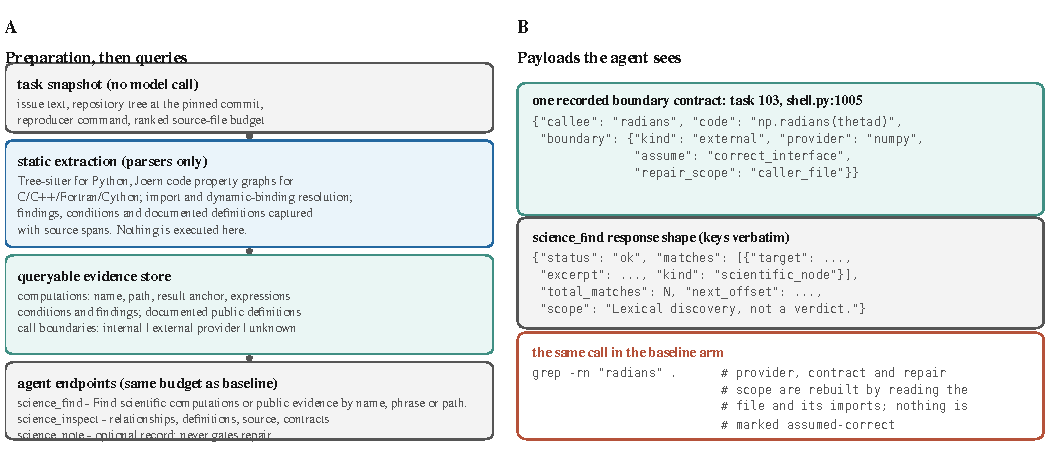
\includegraphics[width=0.77\linewidth]{../figures/out/fig_grounding_flow.pdf}
  \caption{How the representation reaches the agent. Preparation uses parsers and analyzers only ---
  no model call, no execution --- and the agent queries it via \texttt{science\_find},
  \texttt{science\_inspect} and the optional \texttt{science\_note}. The right panel shows recorded
  payloads; the contract excerpt is verbatim from task 103's saved science state, with external
  providers marked \texttt{assume: correct\_interface} and unresolved callees labelled
  \texttt{unknown\_external} rather than guessed.}
  \label{fig:flow}
\end{figure}

\section{What the agent gets}
Preparation runs once per task and never calls a model: files are ranked so execution evidence and
boundary callers precede shallow entry points; Python is parsed with Tree-sitter and C, C++,
Fortran and Cython with Joern code property graphs, with explicit fallback when a frontend is
missing. The store records computations (name, path, result anchor, expressions), governing
conditions and findings, documented public definitions with source spans, and \emph{call
boundaries} of three kinds: internal, external with a named provider, unknown\_external. Across the
94 prepared tasks with frozen bundles the median task yields 296 scientific objects (maximum
10{,}887); boundaries recorded during the held-out science runs comprise 12{,}794 external, 1{,}890
unknown\_external and 534 internal calls. Both arms receive identical shell tools, and every tool
call, model second and reasoning token counts against the same 1800\,s budget.

\section{Protocol}
Thirty development tasks were used for iteration; 89 tasks were locked before the reported runs.
The task-to-domain mapping comes from the benchmark paper's task-level inventory (Appendix
Table~5), re-extracted and validated against its published per-domain counts, so domain strata are
not our annotation. Both arms use DeepSeek V4.1 Flash at temperature $0$ with
\texttt{PYTHONHASHSEED=0}, the same image, budget and verifier; containers run without network and
verifier containers start only after repair terminates, so private tests are never visible. Solve
means official verifier reward; per-attempt private-test fractions are retained as partial credit.
The held-out partition ran three times (534 scheduled, 522 verified attempts), development four
times, and both arms additionally ran at high and low reasoning effort on development
\cite{deepseekusage}. Verifier receipts per attempt are the only source of numbers
(\texttt{analysis/paper\_facts.py} $\rightarrow$ \texttt{results/paper-facts.json}).

\section{Results}
\subsection{Held-out parity at lower output cost}
On the held-out partition the arms solve the same number of attempts --- 60/260 (23.1\%) with
evidence against 60/262 (22.9\%) without --- and the paired comparison over tasks is flat: 74 ties,
7 tasks better with evidence, 8 worse, sign test $p{=}1.00$, bootstrap interval $[-3.4,+4.9]$\,pp.
Development is equally flat (44/118 vs.\ 43/117); pass@3 is 31.5\% against 32.6\%.

The difference is cost, not solves (Fig.~\ref{fig:resources}). The evidence arm emits 10.36M output
tokens against 12.01M, 13.7\% fewer --- 1.65M tokens over 522 verified attempts, at 39.8k instead of
45.8k per attempt --- while uncached input rises modestly (878M vs.\ 838M) because the arm still
reads files; wall-clock work per attempt is 1306.9\,s against 1236.6\,s. Partial credit moves the
other way (70.7\% vs.\ 73.1\% pooled private-test pass rate), consistent with a narrower search
that either finds the right computation or stops short rather than a loss of partial progress.

\begin{table}[t]
\centering
\caption{All numbers regenerate from frozen receipts via \texttt{analysis/paper\_facts.py}.}
\label{tab:main}
\footnotesize
\setlength{\tabcolsep}{3.5pt}
\begin{tabular}{@{}llrrr@{}}
\toprule
& & \textbf{baseline arm} & \textbf{evidence arm} & \textbf{contrast} \\
\midrule
Held-out 89 $k{=}3$ & attempts solved & 60/262 (22.9\%) & 60/260 (23.1\%) & $+0.2$\,pp \\
& paired tasks & \multicolumn{3}{r}{74 ties, 7 evidence-only, 8 baseline-only; sign test $p=1.00$} \\
& output tokens & 12.01M (45.8k/attempt) & 10.36M (39.8k/attempt) & $-13.7\%$ \\
& private tests & 2315/3167 (73.1\%) & 2226/3148 (70.7\%) & $-2.4$\,pp \\
\midrule
Development 30 $k{=}4$ & attempts solved & 43/117 (36.8\%) & 44/118 (37.3\%) & $+0.5$\,pp \\
\midrule
Dev 30 effort matrix & high effort & 12/30 (40.0\%) & 11/30 (36.7\%) & $-3.3$\,pp \\
& low effort & 12/30 (40.0\%) & 13/30 (43.3\%) & $+3.3$\,pp \\
\bottomrule
\end{tabular}
\end{table}

\begin{figure}[tb]
  \centering
  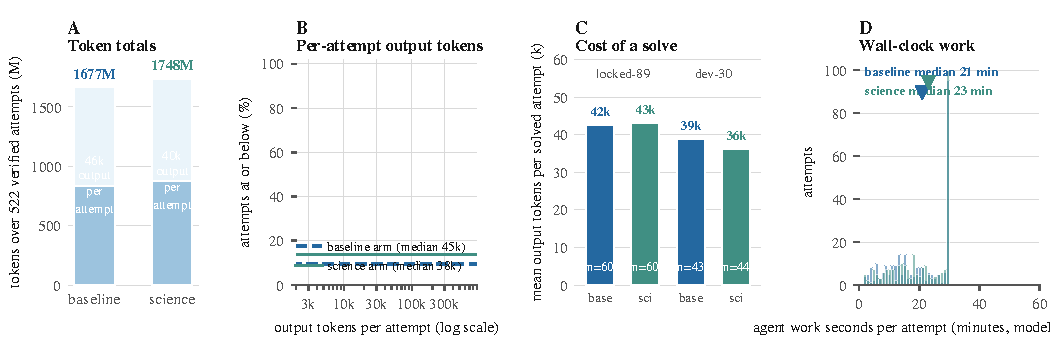
\includegraphics[width=0.73\linewidth]{../figures/out/fig_resources.pdf}
  \caption{Resource use at matched solve rates (522 held-out verified attempts).
  \textbf{A}~pooled token composition; \textbf{B}~per-attempt output-token distributions;
  \textbf{C}~mean output tokens per \emph{solved} attempt on both partitions; \textbf{D}~agent work
  seconds per attempt.}
  \label{fig:resources}
\end{figure}

\subsection{Where the representation helps, and where it hurts}
Aggregate parity hides opposing strata (Fig.~\ref{fig:domains}). Held-out mechanics improves by
22.2\,pp (0/9$\rightarrow$2/9), astronomy by 12.4\,pp (2/14$\rightarrow$4/15), materials science and
engineering by 9.7\,pp (8/44$\rightarrow$12/43) and civil engineering by 6.7\,pp; biomedical
engineering falls 16.7\,pp (13/30$\rightarrow$8/30) and biology 9.5\,pp
(7/18$\rightarrow$5/17); chemistry (19 tasks), physics (7) and mathematics (5) are exactly
unchanged. Development shows the same texture: mathematics gains 37.5\,pp (0/8$\rightarrow$3/8) and
statistics 25\,pp, while chemistry loses 10\,pp.

The discordant task IDs name the mechanism. Held-out wins for the evidence arm are 020, 042, 074,
103 and 116; losses are 022, 029, 053, 063, 087 and 093. Task 103 (pyNastran, symmetric composite
laminate ABD calculations) is solved 2 of 3 times with evidence and 0 of 3 without, and its saved
state shows the arm inspecting the ply-angle computation and its \texttt{numpy} boundaries instead
of scanning parser code. Task 022 (nilearn, volume-to-surface projection) is the mirror image:
2 of 3 with the baseline, 0 of 3 with evidence, with the trajectory reading projection mathematics
before touching the atlas label mapping the instructions actually concern. That is the split:
strata that improve are ones where the defect \emph{is} a computation, strata that degrade are ones
where an ordinary software defect sits under scientific prose.

Stratifying by the benchmark's knowledge-ablation flag gives $-$0.3\,pp for ablated tasks
(47/188 vs.\ 48/190) and $+1.4$\,pp for knowledge-provided tasks (13/72 vs.\ 12/72): no detectable
interaction. Language strata are uninformative here --- 81 of 89 locked tasks are pure Python, and
the ten multi-language tasks were solved by neither arm except two pure-C tasks solved by both.

\begin{figure}[tb]
  \centering
  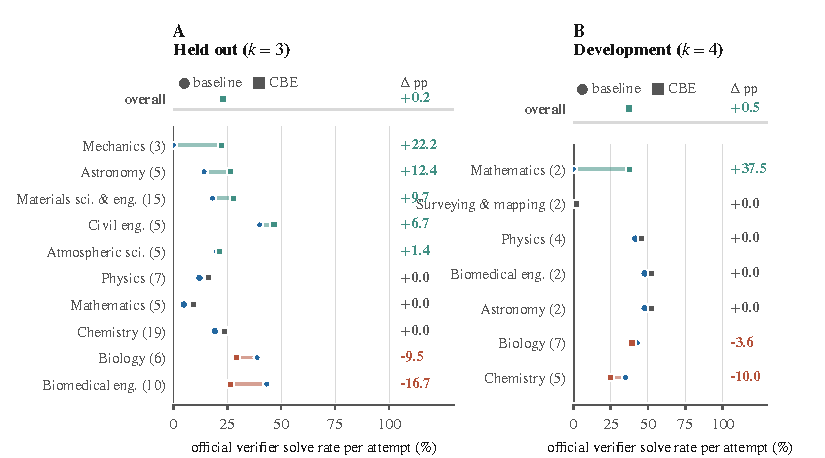
\includegraphics[width=0.79\linewidth]{../figures/out/fig_domains.pdf}
  \caption{Domain outcome map (\texttt{results/domain-arm-analysis.json}). Rows appear where the
  partition holds at least three (locked, \textbf{A}) or two (development, \textbf{B}) tasks;
  circles mark the baseline arm, squares the evidence arm, whiskers its Wilson 95\% interval and the
  right column the difference.}
  \label{fig:domains}
\end{figure}

\subsection{Replication structure dominates}
Three held-out replicates make the measurement problem explicit (Fig.~\ref{fig:stability}): per
arm, 60 (baseline) and 61 (evidence) tasks are never solved, 11 and 10 are solved by every
replicate, and 18 tasks flip inside each arm. The joint distribution sits on the diagonal --- 55
tasks at 0/0 and 10 at 3/3 --- with only 15 tasks disagreeing between arms at all. Since about a
fifth of tasks move under identical conditions, a single-run difference of 1--3\,pp carries no
signal; that is why we report raw counts beside every percentage.

\subsection{Reasoning effort substitutes for evidence}
At high reasoning effort the baseline leads development 12/30 against 11/30; at low effort the
evidence arm leads 13/30 against 12/30. On the 20-task subset evaluated at both levels the
high-effort evidence deficit (8/20 vs.\ 10/20) disappears (10/20 vs.\ 10/20), and the two tasks it
recovered at low effort (002, 009) are exactly the two it lost at high effort --- the signature of
external structure standing in for deliberation. Tool use in that subset: 61
\texttt{science\_inspect}, 10 \texttt{science\_find}, 20 records over 20 tasks.

\begin{figure}[tb]
  \centering
  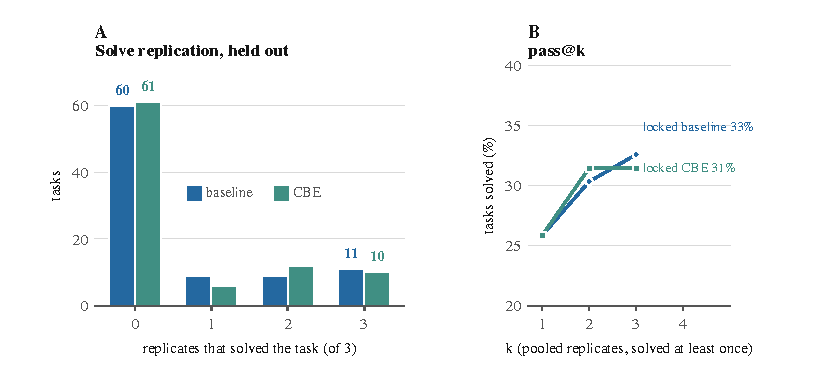
\includegraphics[width=0.75\linewidth]{../figures/out/fig_stability.pdf}
  \caption{Replicate structure of the held-out partition. \textbf{A}~tasks by number of replicate
  runs that solved them; \textbf{B}~pass@$k$ curves; \textbf{C}~per-task solve-rate pairing with
  one-arm-only counts annotated.}
  \label{fig:stability}
\end{figure}

\section{Threats and conclusion}
\textbf{Threats.} One model and one budget bound every result: a different model, or a budget that
lets the baseline exhaust its search, could move both the parity line and the domain split.
Individual domain rows --- single-task rows and the $k{=}1$ effort cells especially --- are
descriptive, and only the aggregate held-out comparison is inferential. Unparseable expressions are
recorded as unsupported and external calls are treated as assumed-correct interfaces, so a
misclassification would silently remove a file from scope. Development tasks are optimistic by
construction; the locked partition alone supports the parity claim.

A queryable account of scientific structure changed repair behaviour without changing average solve
rate: parity on 522 held-out verified attempts, 13.7\% fewer generated tokens, and a domain-dependent split
in which computation-shaped defects improve by up to 22\,pp while software-shaped defects under
scientific prose degrade by up to 17\,pp. Context about science is not a uniform prior; it is a lens
that sharpens some tasks and distorts others, and the benchmark's replicate structure makes the
difference measurable only at $k\ge3$.

\clearpage
\section*{Artifacts, provenance and division of work}
Code, receipts and figures are in the submission repository (URL and commit hash in
\texttt{README.md} and \texttt{REPRODUCTION.md}); the reported 757 verified attempts total 115/379 for the
baseline and 117/378 with evidence. Every number here regenerates from \texttt{analysis/paper\_facts.py}
into \texttt{results/paper-facts.json}, and every figure renders from frozen receipts through
\texttt{paper/figures/make\_all.py} with a layout assertion before writing. Task IDs are benchmark
IDs and domain labels are the benchmark paper's domains. Rajarshi Ghoshal designed the
representation, protocol and analysis and wrote this report; LLM coding assistants implemented
harness plumbing, parsers and figures and helped revise prose. DeepSeek V4.1 Flash was the only
model used for repair attempts, and the development partition was the only basis for iteration. No
prior research of the author is claimed as the basis of this method.

\begin{samepage}
\begin{thebibliography}{9}

\bibitem[Xu et al.(2026)]{xu2026swebenchscience}
Z.~Xu, J.~Lu, Y.~Zheng, Y.~Wang, and X.~Qiu.
\newblock SWE-bench Science: can coding agents resolve engineering tasks in science?
\newblock \emph{arXiv preprint arXiv:2608.19799v2}, 2026.

\bibitem[Jimenez et al.(2024)]{jimenez2024swebench}
C.~E. Jimenez, J.~Yang, A.~Wettig, S.~Yao, K.~Pei, O.~Press, and K.~Narasimhan.
\newblock SWE-bench: can language models resolve real-world GitHub issues?
\newblock In \emph{International Conference on Learning Representations (ICLR)}, 2024.

\bibitem[Niu et al.(2023a)]{niu2023ablots}
F.~Niu, C.~Mayr-Dorn, W.~K.~G. Assun{\c{c}}{\~a}o, L.~Huang, J.~Ge, B.~Luo, and A.~Egyed.
\newblock The ABLoTS approach for bug localization: is it replicable and generalizable?
\newblock In \emph{Proc.\ 20th International Conference on Mining Software Repositories (MSR)},
pp.~152--162, 2023.

\bibitem[Niu et al.(2023b)]{niu2023rat}
F.~Niu, W.~K.~G. Assun{\c{c}}{\~a}o, L.~Huang, C.~Mayr-Dorn, J.~Ge, B.~Luo, and A.~Egyed.
\newblock RAT: a refactoring-aware traceability model for bug localization.
\newblock In \emph{Proc.\ 45th International Conference on Software Engineering (ICSE)}, 2023.

\bibitem[Niu et al.(2025)]{niu2025tvr}
F.~Niu, L.~Huang, C.~Mayr-Dorn, and A.~Egyed.
\newblock TVR: automotive system requirement traceability validation and recovery through
retrieval-augmented generation.
\newblock \emph{arXiv preprint arXiv:2504.15427}, 2025.

\bibitem[Pan et al.(2025)]{pan2025coverage}
X.~Pan, F.~Niu, L.~Huang, and A.~Egyed.
\newblock Requirements coverage-guided minimization for natural language test cases.
\newblock \emph{arXiv preprint arXiv:2505.20004}, 2025.

\bibitem[{ML4AI Team}(2024)]{skema2024gromet}
ML4AI Team.
\newblock GroMEt: a unified intermediate representation for scientific models and code.
\newblock DARPA ASKEM / SKEMA consortium, 2024.

\bibitem[Hein et al.(2020)]{automates2020}
P.~Hein et~al.
\newblock AutoMATES: automated model assembly from text, equations and software.
\newblock \emph{arXiv preprint arXiv:2001.07295}, 2020.

\bibitem[Yamaguchi et al.(2014)]{yamaguchi2014cpg}
F.~Yamaguchi, N.~Golde, D.~Arp, and K.~Rieck.
\newblock Modeling and discovering vulnerabilities with code property graphs.
\newblock In \emph{IEEE Symposium on Security and Privacy (S\&P)}, 2014.

\bibitem[Brunsfeld et al.(2024)]{treesitter}
M.~Brunsfeld et~al.
\newblock Tree-sitter: an incremental parsing system for programming tools.
\newblock \url{https://tree-sitter.github.io}, 2024.

\bibitem[DeepSeek(2026)]{deepseekusage}
DeepSeek.
\newblock DeepSeek V4.1 Flash API documentation: reasoning-effort parameter.
\newblock \url{https://api-docs.deepseek.com}, 2026.

\end{thebibliography}
\end{samepage}

\end{document}
